\documentclass[12pt]{article}

\usepackage{graphicx}
\graphicspath{ {/home/gerardo/Documentos/Gera/SyntheticBiobots/2022/Metods/Docking/1/Transripts} }
\usepackage{hyperref}
\usepackage{placeins}
\usepackage{fancyhdr}
\pagestyle{fancy}
\lhead{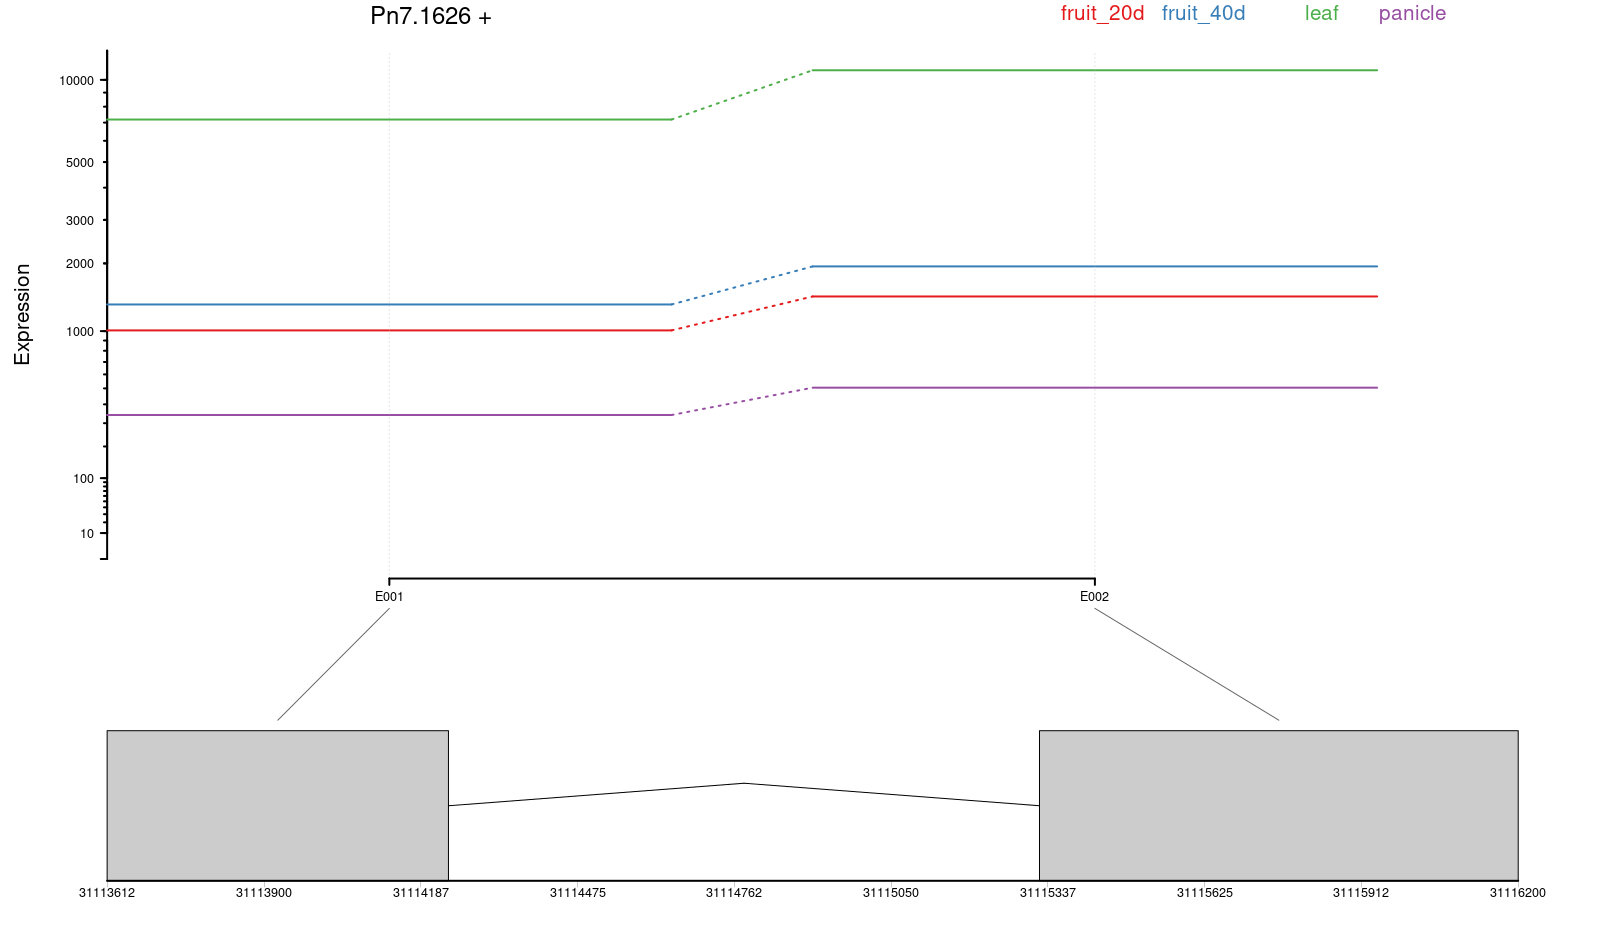
\includegraphics[width=.06\textwidth]{1.png}}
\rhead{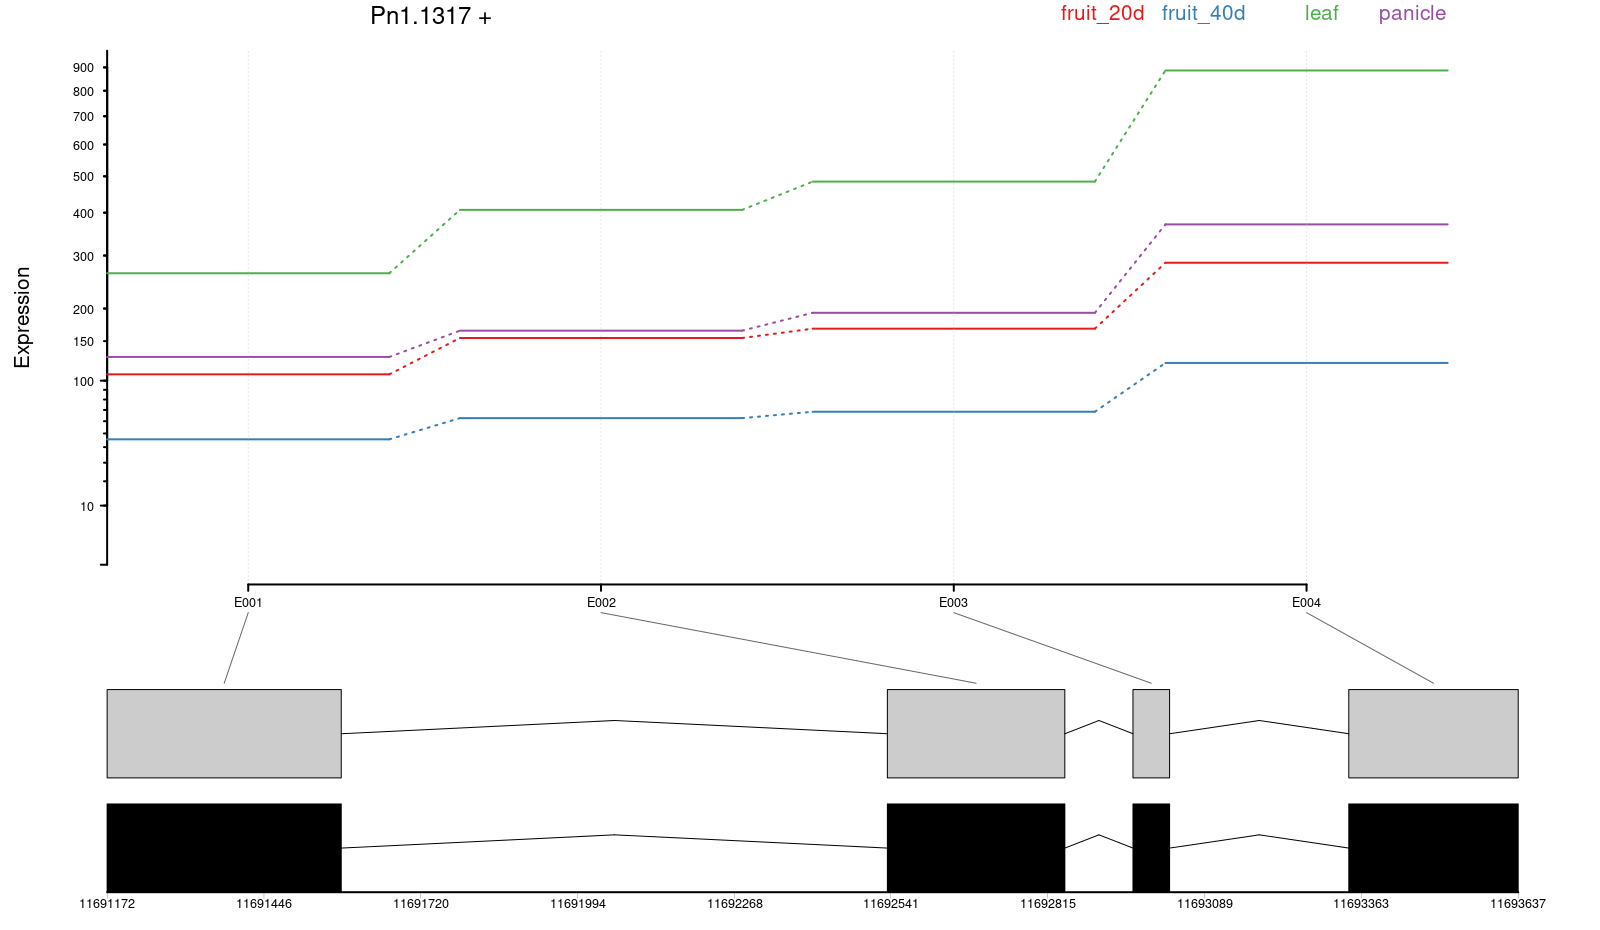
\includegraphics[width=.06\textwidth]{2.png}}
\usepackage[left=1.8cm,top=2.54cm,right=1.8cm,bottom=2.54cm,bindingoffset=0.5cm]{geometry}
\usepackage{natbib}

\begin{document}
	\renewcommand{\figurename}{Figura}
	
	\title {Módulo 8: Actividad 2\\Ciclo de la Urea}
	\date{28 Noviembre 2021}
	\author{Gerardo Cendejas Mendoza\\ Facultad de Ciencias UNAM\\BMC II}
	
	\maketitle
	
	El ciclo de la Urea y el ciclo de Krebs están interrelacionados mediante un sistema llamado ``lanzadera Aspartato--Malato". Esta lanzadera se llama así debido a los dos intermediarios aspartato y malato, son transportados desde el interior y hacia el exterior de la mitocondria, respectivamente. Ninguno de éstos dos intermediarios pertenecen ni a Krebs ni a Urea. Explica ¿cómo es que se relacionan el ciclo de Krebs y el de la Urea a través de éstos intermediarios?
	
	\FloatBarrier
	\begin{figure}[h]
		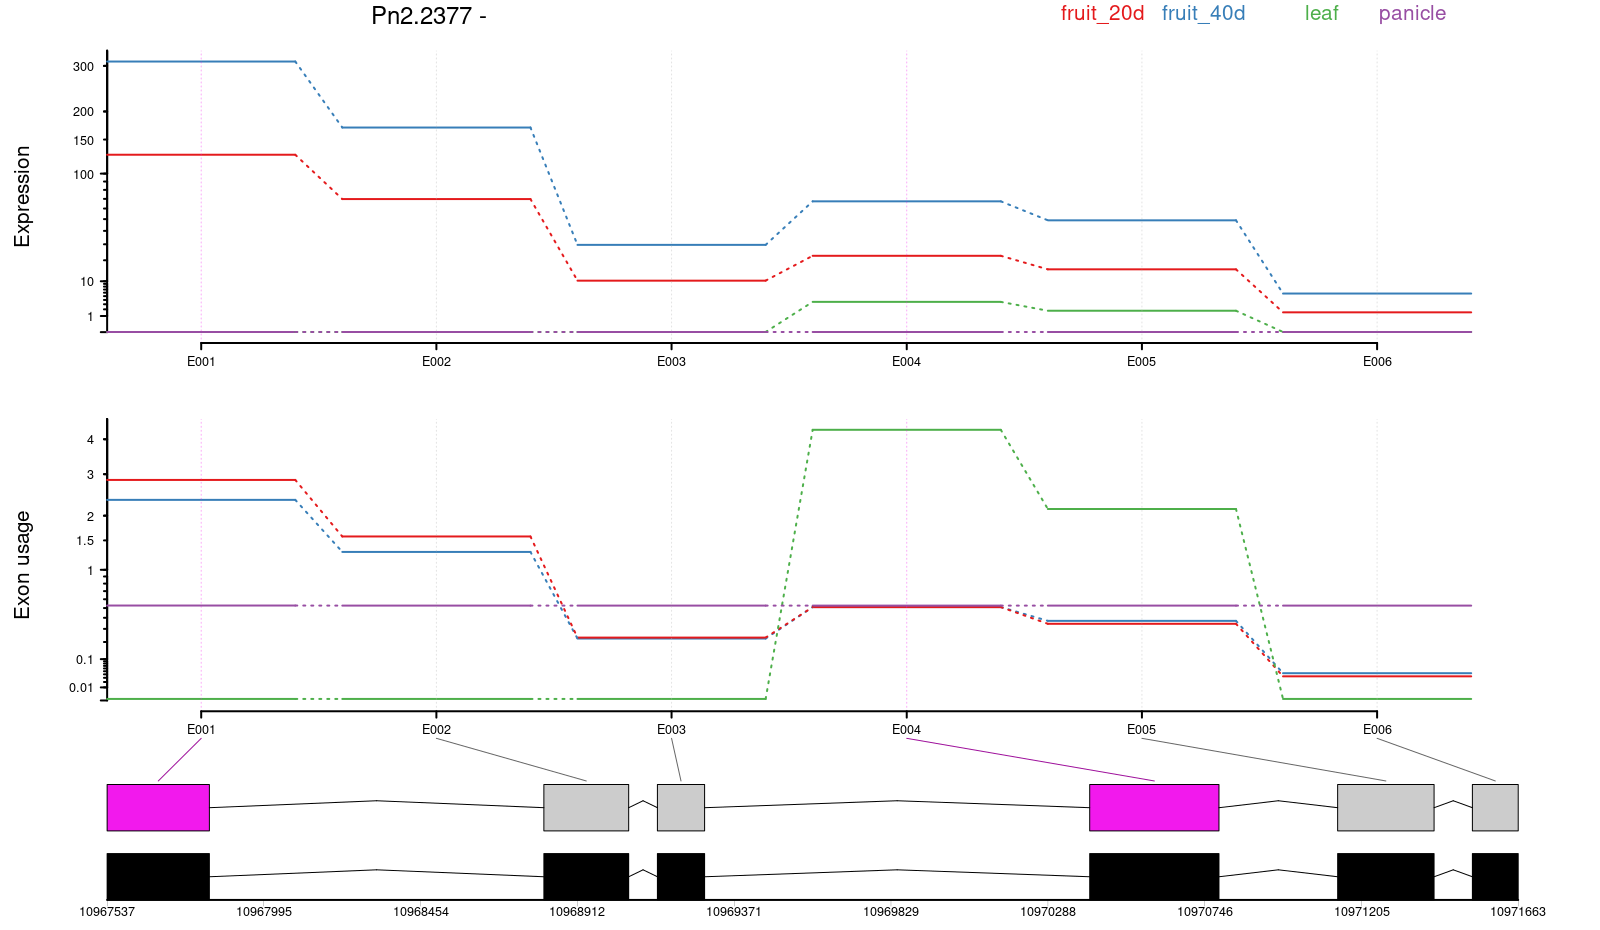
\includegraphics[scale=0.4]{../../2/Transcripts/7.png}
	\end{figure}
	\FloatBarrier
	
	\newpage
	
	El ciclo de Krebs y el ciclo de la urea se relacionan porque en la mitocondria y en el citoplasma se encuentran isoenzimas que llevan a cabo las mismaas reacciones, de convertir fumarato a malato, este a oxalacetato y este a aspartato. Además, como resultado del ciclo de la urea se obtiene fumarato, que es un intermediario del ciclo de Krebs y mediante la lanzadera de Apartato--Malato puede entrar a la matriz mitocondrial y entrar al ciclo de Krebs. De igual manera, a partir del oxalacetato del ciclo de Krebs se puede generar Aspartato, el cual por la misma lanzadera puede salir de la mitocondria y llegar al citosol, aquí puede entrar al ciclo de la urea, pues es necesario en este para la obtención de arginosuccinato a partir de citrulina.
	
\end{document}